%%%%%%%%%%%%%%%%%%%%%%%%%%%%%%%%%%%%%%%%%%%%%%%%%%%%%%%%%%%%%%%%%%%%%%%%%%%
%% This file is part of the book
%%
%% Algorithmic Graph Theory
%% http://code.google.com/p/graph-theory-algorithms-book/
%%
%% Copyright (C) 2009--2011 Minh Van Nguyen <nguyenminh2@gmail.com>
%%
%% See the file COPYING for copying conditions.
%%%%%%%%%%%%%%%%%%%%%%%%%%%%%%%%%%%%%%%%%%%%%%%%%%%%%%%%%%%%%%%%%%%%%%%%%%%

\documentclass{article}

\usepackage{subfigure}
\usepackage{tikz}
\usetikzlibrary{external}
\tikzexternalize{bipartite-complete-bipartite-graphs}

\begin{document}

\begin{figure}
%% bipartite graph
\subfigure[Bipartite]{
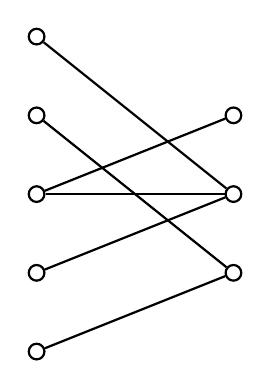
\begin{tikzpicture}
[nodeDecorate/.style={shape=circle,inner sep=2pt,draw,thick},%
  lineDecorate/.style={-,thick}]
%% nodes or vertices
\foreach \nodename/\x/\y in {
  a/0/0, b/0/1, c/0/2, d/0/3, e/0/4, f/2.5/3, g/2.5/2, h/2.5/1}
{
  \node (\nodename) at (\x,\y) [nodeDecorate] {};
}
%% edges or lines
\path
\foreach \startnode/\endnode in {a/h, b/g, c/g, c/f, d/h, e/g}
{
  (\startnode) edge[lineDecorate] node {} (\endnode)
};
\end{tikzpicture}
}
%%
%%
\quad
%% complete bipartite graph K_{4,3}
\subfigure[$K_{4,3}$]{
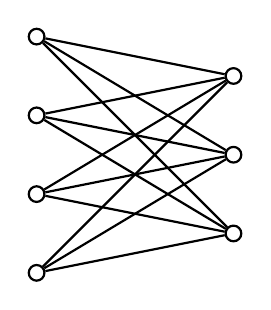
\begin{tikzpicture}
[nodeDecorate/.style={shape=circle,inner sep=2pt,draw,thick},%
  lineDecorate/.style={-,thick}]
%% nodes or vertices
\foreach \nodename/\x/\y in {
  a/0/0, b/0/1, c/0/2, d/0/3, e/2.5/2.5, f/2.5/1.5, g/2.5/0.5}
{
  \node (\nodename) at (\x,\y) [nodeDecorate] {};
}
%% edges or lines
\path
\foreach \startnode/\endnode in {
  a/e, a/f, a/g, b/e, b/f, b/g, c/e, c/f, c/g, d/e, d/f, d/g}
{
  (\startnode) edge[lineDecorate] node {} (\endnode)
};
\end{tikzpicture}
}
%%
%%
\quad
%% complete bipartite graph K_{3,3}
\subfigure[$K_{3,3}$]{
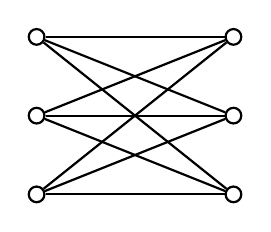
\begin{tikzpicture}
[nodeDecorate/.style={shape=circle,inner sep=2pt,draw,thick},%
  lineDecorate/.style={-,thick}]
%% nodes or vertices
\foreach \nodename/\x/\y in {
  a/0/0, b/0/1, c/0/2, d/2.5/2, e/2.5/1, f/2.5/0}
{
  \node (\nodename) at (\x,\y) [nodeDecorate] {};
}
%% edges or lines
\path
\foreach \startnode/\endnode in {
  a/d, a/e, a/f, b/d, b/e, b/f, c/d, c/e, c/f}
{
  (\startnode) edge[lineDecorate] node {} (\endnode)
};
\end{tikzpicture}
}
%%
%%
\quad
%% star graph K_{1,4}
\subfigure[$K_{1,4}$]{
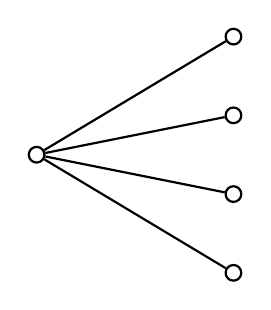
\begin{tikzpicture}
[nodeDecorate/.style={shape=circle,inner sep=2pt,draw,thick},%
  lineDecorate/.style={-,thick}]
%% nodes or vertices
\foreach \nodename/\x/\y in {
  a/0/1.5, b/2.5/3, c/2.5/2, d/2.5/1, e/2.5/0}
{
  \node (\nodename) at (\x,\y) [nodeDecorate] {};
}
%% edges or lines
\path
\foreach \startnode/\endnode in {a/b, a/c, a/d, a/e}
{
  (\startnode) edge[lineDecorate] node {} (\endnode)
};
\end{tikzpicture}
}
\end{figure}

\end{document}
